\cleardoublepage\documentclass[../main.tex]{subfiles}
\begin{document}
\renewcommand\contentsname{Conteúdos do Capítulo}
\chapter{Aplicações da integração}\label{cap:apl_integracao}\index{aplicações! integrais}
\minitoc
%\tableofcontents
\subsection*{Objetivos de aprendizagem do capítulo}
\addcontentsline{toc}{section}{Objetivos de aprendizagem do capítulo}
Ao final deste capítulo você deverá ser capaz de:
\begin{itemize}
    \item \item Interpretar corretamente a integral definida na aplicação do cálculo de áreas de regiões planas, volume, comprimento de arco, etc.
\end{itemize}
\section{Área entre Curvas}
%\subsection{Áreas limitadas por curvas da forma \normalsize{$y=f(x)$ e $y=g(x)$}}
\figtext{0.7cm}{l}{0.45}{%
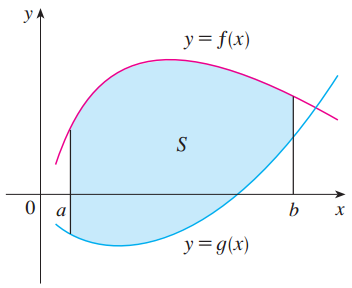
\includegraphics[width=7cm]{figs/AreaEntcurvas/AreaCuvas}
\vspace{-0.8cm}
\captionof{figure}{\\\footnotesize{$S=\{s (x, y) |a\leq x\leq b, g(x)\leq y\leq f(x)\}$}}
\label{fig:AreaCurvas}
}%

\noindent No Capítulo \ref{cap:IntDef} definimos e calculamos áreas de regiões sob gráficos de funções. Aqui, usaremos as integrais para encontrar áreas de regiões entre gráficos de duas funções.

\noindent Considere a região S delimitada por duas curvas $y=  f ( x )$ e $y = g ( x )$ e pelas retas
verticais \(x =a\) e \(x=  b \), onde \(f\) e $g$ são funções contínuas e \(f ( x ) \geq g ( x ) \) para todo \(x\) em \([a, b]\). (Veja a Fig. \ref{fig:AreaCurvas}).

\noindent Assim como fizemos para as áreas sob as curvas na Seção \ref{subsec:SomaRiemann}, podemos dividir $S$ em $n$ faixas de larguras iguais e então aproximamos a i -ésima faixa por um retângulo com base $\Delta x$ e altura $f(x_i^*)-g(x_i^*)$ \cite{StwartVol17ed}, o que nos leva a deduzir que a área entre duas curvas conforme figura \ref{fig:AreaCurvas}, é dada como segue. 
\vspace{-0.4cm}
\begin{framed}
\vspace{-0.3cm}
\begin{definition}
 A área $A$ da região limitada pelas curvas $y= f ( x)$, $y= g ( x)$ e pelas retas $x  =a$, 
$x  =b$ , onde $f$ e $g$ são contínuas e $f (x ) \geq  g ( x )$ para todo $x$ em $[a, b]$, é
\begin{equation}
    A=\int_a^b\pr{f(x)-g(x)}\, dx\label{eq:AreaCurvas}
\end{equation}
\end{definition}\vspace{-0.45cm}
\end{framed}
\vspace{-0.5cm}

\begin{ex}~
Encontre a área da região limitada acima por $y=e^x$, limitada abaixo por $y=x$, e limitada nos lados por $x=0$ e $x=1$.

\begin{solut}~
%\vspace{-0.3cm}
\pichskip{0.2cm}%distância entre texto e figura
\parpic[r]{%\includegraphics[scale=0.75]{cap_apl_integracao/figs/AreaEntcurvas/AreaEntreFuncSenCos.png}}
\begin{minipage}{0.2\textwidth}
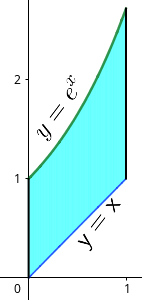
\includegraphics[scale=0.65]{figs/AreaEntcurvas/AreaExp-y=x.png}
\captionof{figure}{}%
\label{fig:AreaExp-y=x}
\end{minipage}
}
\noindent A região é mostrada na Figura \ref{fig:AreaExp-y=x}. A curva limitante superior é $y=e^x$ e a curva limitante inferior é $y=x$. Então, usamos a fórmula da área \ref{eq:AreaCurvas} com $f(x )=  e^x$, $g ( x )=  x$, $a=  0$ e $b= 1$:
\begin{align*}
    A&=\intg{e^x-x}\\&=\left.e^x-\frac{1}{2}x^2\right]_0^1\\&=e-\frac{1}{2}-1\\&=e-1,5
\end{align*}
\end{solut}
\end{ex}

\begin{ex}
Encontre a área delimitada pelos gráficos de $y = 3 - x$ e $y = x^2 - 9$. (Veja a Figura \ref{fig:AreaEntreCurvasEx2}).\\
\begin{figure}[h!tb]
    \centering
    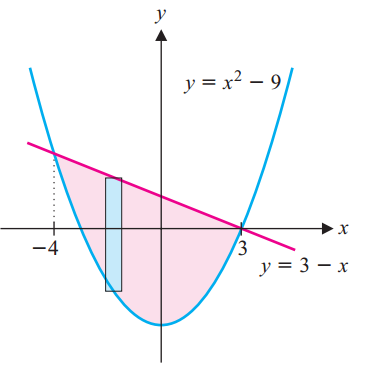
\includegraphics[scale=0.75]{figs/AreaEntcurvas/AreaEntreCurvasEx}
    \caption{}
    \label{fig:AreaEntreCurvasEx2}
\end{figure}
\begin{solut}~
A região na Figura \ref{fig:AreaEntreCurvasEx2} é determinada pela interseção das duas curvas. Os limites da integração corresponderão então às coordenadas $x$ dos pontos de interseção. Para encontrar os limites, definimos as duas funções iguais e resolvemos para $x$, da seguinte forma:\\
 \centerline{$3- x = x^2 - 9$ ou $0 = x^2 + x - 12 = ( x - 3)(x + 4)$}
 
 Assim, as curvas se interceptam em $x = -4$ e $x = 3$. Tenha cuidado para observar no gráfico qual curva forma o limite superior da região e qual forma o limite inferior fronteira. Nesse caso, o limite superior é formado por $y = 3 - x$. Então, para cada fixo valor de $x$, a altura de um retângulo (como a indicada na Figura \ref{fig:AreaEntreCurvasEx2}) é
$$h ( x ) = (3 - x ) - ( x^2 - 9)$$
De \ref{eq:AreaCurvas},  á área entre as curvas dadas é
\begin{align*}
  A&=\intdef{-4}{3}{\pr{(3-x)-(x^2-9)}}\\
  & = \intdef{-4}{3}{-x^2-x+12}\\
  &=\pr{-\frac{x^2}{3}-\frac{-x^2}{2}+12x}_{-4}^3=\frac{343}{6}%
\end{align*}
%\vspace{-0.5cm}
\end{solut}
\end{ex}
\begin{ex}
Encontre a área da região delimitada pelas parábolas $y =x^2$ e $y = 2 x - x^2$.
\end{ex}
\solution
\begin{wrapfigure}[9]{r}{0.4\textwidth}
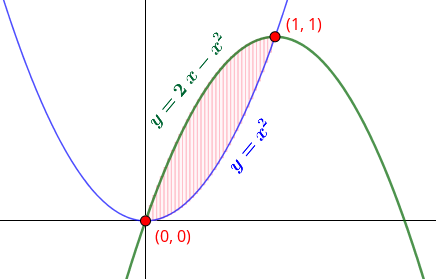
\includegraphics[width=0.4\textwidth]{figs/AreaEntcurvas/AreaCurvasEx3.png}
\caption{}\label{fig:eAreaCurvasx3}
\end{wrapfigure}
 Primeiro encontramos os pontos de intersecção das parábolas, resolvendo suas equações simultaneamente. Isso resulta em $ x^2=  2 x- x^2$ ou $2x^2 - 2 x=  0$. Portanto, $2 x ( x - 1)=  0$, então $x=0$ ou $x=1$. Os pontos de intersecção são $(0, 0)$ e $(1, 1)$.  Vemos na Figura \ref{fig:eAreaCurvasx3} que $2x-x^2\geq x^2$ entre os pontos de intersecção.
 
 Assim, a área da região delimitada por estas curvas é dada por
\begin{align*}
    \intdef{0}{1}{(2x-2x^2)}&=2\intdef{0}{1}{(x-x^2)}\\
& =2\pr{\frac{x^2}{2}-\frac{x^3}{3}}_0^1=2\pc{\frac{1}{2}-\frac{1}{3}}=\frac{1}{3}
\end{align*}
%\vspace{-0.5cm}
\hrule
\vspace{0.3cm}
\minipag{0.5}{
Para encontrarmos a área entre as curvas $y=f(x)$ e $y=g(x)$ onde $f(x)\geq g(x)$ para alguns valores de $x$, mas $g(x)\geq f(x)$ para outros valores de $x$ , então dividimos determinada região $S$ em várias regiões $S$1 , $S$2 , com áreas $A_1 , A_2, \ldots$, como mostrado na Figura \ref{fig:AreaPartesdeCurvas}. Em seguida, definimos a área da região $S$ como a soma das áreas das regiões menores $S_1 , S _2 ,\ldots$, ou seja, $A=A_1+A_2+\ldots$. Uma vez que\\
}\hfill
\minipag{0.47}{%
    \centering
    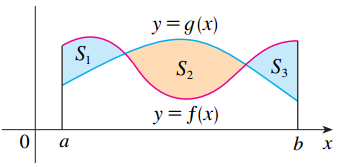
\includegraphics[width=8cm]{figs/AreaEntcurvas/AreaPartesdeCurvas.png}
    \vspace{-1.2cm}
    \captionof{figure}{}%
    \label{fig:AreaPartesdeCurvas}
}%
\matt{
|f(x)-g(x)=\begin{cases}
f(x)-g(x) \quad \textrm{ onde } f(x)\geq g(x)\\
g(x)-f(x) \quad\textrm{ onde } g(x)\geq f(x)
\end{cases}
}
temos a seguinte expressão para $A$.
\begin{framed}
\vspace{-0.2cm}
\begin{definition}
    A área entre as curvas $y=f(x)$ e $y=g(x)$ e entre $x=a$   e $x=b$   é
\begin{equation}
    A=\intdef{a}{b}{|f(x)-g(x)|}\label{eq:IntdoMod}
    \end{equation}
\end{definition}
\end{framed}
Quando calculamos a integral em \ref{eq:IntdoMod}, no entanto, ainda temos que dividi-la em integrais
correspondentes a $A_1, A_2,\ldots$.
\begin{ex}
Encontre a área da região delimitada pelas curvas $y=\sin x, y=\cos x, x=0$,  e $x=\pi/2$.

\begin{solut}~
\pichskip{0.2cm}%distância entre texto e figura
\parpic[r][b]{%\includegraphics[scale=0.75]{cap_apl_integracao/figs/AreaEntcurvas/AreaEntreFuncSenCos.png}}
\begin{minipage}{0.45\textwidth}
\includegraphics[scale=0.75]{figs/AreaEntcurvas/AreaEntreFuncSenCos.png}
\captionof{figure}{}
\label{fig:AreaEntreFuncSenCos}
\end{minipage}
}%
\noindent Os pontos de intersecção ocorrem quando $\sen x=\cos x x$, isto é, quando $x=\pi/4$ (considerando que $0\leq x\leq \pi/2$). A região é esboçada na Figura \ref{fig:AreaEntreFuncSenCos}. Observe que
quando, mas quando Portanto, a área requerida é
\begin{align*}
    A&=\intdef{0}{\pi/2}{|\cos x x-\sin x|}=A_1+A_2\\
    &=\intdef{0}{\pi/4}{\pc{\cos x x-\sin x}}\\
    &+\intdef{\pi/4}{\pi/2}{\pc{\sin x-\cos x x}}\\
    &=\pr{\sin x+\cos x x}_0^{\pi/4}+\pr{-\cos x x-\sin x}_{\pi/4}^{\pi/2}\\
    &=\pc{\frac{1}{\sqrt{2}}+\frac{1}{\sqrt{2}}-0-1}+\pc{0-1+\frac{1}{\sqrt{2}}+\frac{1}{\sqrt{2}}}=2\sqrt{2}-2
\end{align*}
\end{solut}
\end{ex}
\nota{
Neste último exemplo particular, poderíamos ter economizado algum trabalho por perceber que a região é simétrica em torno de $x=\pi/4$ e, assim,
\matt{
A=2A_1=2\intdef{0}{\pi/4}{(\cos x x-\sin x)}
}
}

\subsection*{Área limitada por curvas da forma $x=f(y)$ e $x=g(y)$}
Algumas regiões são mais bem tratadas considerando $x$ como uma função de $y$. Se uma região é delimitada por curvas com equações $x=f(y)$, $x=g(y)$, $y=c$ e $y=d$ , em que $f$ e $g$ são contínuas e $f(y)\geq g(y)$ para $c\geq y\geq d$ (veja a Figura \ref{y=c-y=d}), então sua área é
\begin{equation}
    A=\int_c^d \pr{f(y)-g(y)}\, dy
\end{equation}
\begin{figure}[H]
\center
\subfigure[teste][]{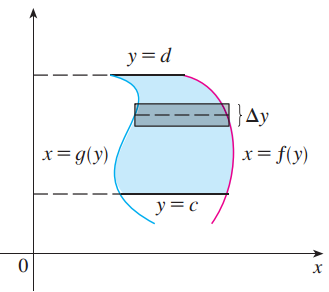
\includegraphics[width=6.7cm]
{figs/AreaEntcurvas/Area-em-func-y1.png}
\label{y=c-y=d}
}
\qquad
\subfigure[b][]{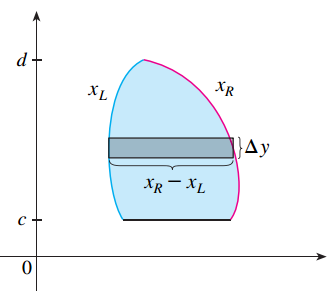
\includegraphics[width=6.7cm]
{figs/AreaEntcurvas/Area-em-func-y2.png}
\label{XR-XL}
}
\caption{Representação de área limitada por curvas da forma $x=f(y)$ e $x=g(y)$}
\label{fig:Area-entre-curvas-x=fy-gy}
\end{figure}

Se escrevermos para o limite à direita e para o limite à esquerda, então, como ilustra a Figura \ref{XR-XL}, teremos
\matt{
A=\int_{c}^d \pr{f(y)-g(y)}\, dy
}

Aqui um retângulo de aproximante típico tem dimensões $X_R-X_L$ e $\Delta y$.

\begin{ex}\label{ex:x=f(y)-x=g(y)}
Encontre a área delimitada pela reta $y=  x - 1$ e pela parábola $y^2=  2 x+6$

\begin{solut}~
\pichskip{0.2cm}%distância entre texto e figura
\parpic[r]{%\includegraphics[scale=0.75]{cap_apl_integracao/figs/AreaEntcurvas/AreaEntreFuncSenCos.png}}
\begin{minipage}{0.3\textwidth}
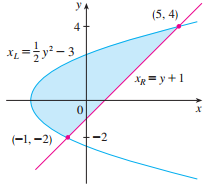
\includegraphics[scale=0.85]{figs/AreaEntcurvas/x=fy-gy-ex}
\captionof{figure}{}%
\label{fig:x=fy-gy}
\end{minipage}
}%
Ao resolvermos as duas equações, vemos que os pontos de intersecção são $( - 1, - 2)$ e $(5, 4)$. Isolamos $x$ na equação da parábola e observamos pela Figura \ref{fig:x=fy-gy} que as curvas de fronteira à esquerda e à direita são\\
\centerline{$x_L=\frac{1}{2}y^2-3$ e $x_R=y+1$}

Devemos integrar entre os valores apropriados de $y =-2$ e $y=  4$. Logo,

\pichskip{0.2cm}%distância entre texto e figura
\parpic[r]{%\includegraphics[scale=0.75]{cap_apl_integracao/figs/AreaEntcurvas/AreaEntreFuncSenCos.png}}
\begin{minipage}{0.4\textwidth}
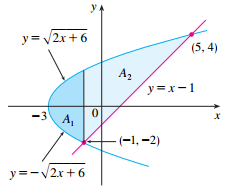
\includegraphics[scale=0.95]{figs/AreaEntcurvas/x=fy-gy-ex-OBS.png}
\captionof{figure}{}%
\label{fig:x=fy-gy-obs}
\end{minipage}
}
\vspace{-1cm}
\begin{align*}
    A&=\int_{-2}^4 \pr{f(y)-g(y)}\, dy\\
    &=\int_{-2}^4 \pr{(y+1)-pc{\frac{1}{2}y-3}}\, dy\\
    &=\int_{-2}^4 \pc{-\frac{1}{2}y^2+y+4}\, dy\\
    &=-\left.\frac{1}{2}\pc{\frac{y^3}{3}}+\frac{y^2}{2}+4y\right]_{-2}^4\\
    &=-\frac{1}{6}\cdot 64+8+16-\pc{\frac{4}{3}+2-8}=18
\end{align*}
\end{solut}
\end{ex}
\nota{
Poderíamos ter encontrado a área no Exemplo \ref{ex:x=f(y)-x=g(y)}, integrando em relação a $x$ em vez de $y$, mas o cálculo é muito mais complicado. Isso significaria dividir a região em duas e calcular as áreas marcadas $A_1$ e $A_2$ na Figura \ref{fig:x=fy-gy-obs}. O método que usamos no Exemplo \ref{ex:x=f(y)-x=g(y)} é muito mais fácil.
}

\subsection{Exercícios resolvidos}
\begin{exeresol}
Calculemos a área da região R limitada por:
\begin{compactenum}[a)]
\item A parábola \(y=4x-x^2\) e o eixo \(x\).

\begin{solution}
Como \(y=4x-x^2\), logo, \(y-4=-(x-2)^2\) é uma parábola de vértice no ponto \((2,4)\) (veja o item (a) da figura a seguir). Logo,

\[ A_R= \mathlarger{\int}^{4}_{0} y\,dx = \mathlarger{\int}^{4}_{0} (4x-x^2)\,dx= \left(2x^2- \dfrac{x^3}{3} \right)\Big{|}^{4}_{0} = \dfrac{32}{4}^2. \]
\end{solution}
\begin{figure}[H]
\centering
\subfigure[teste][]{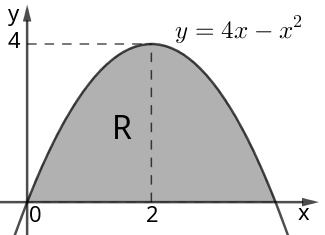
\includegraphics[width=0.36\textwidth]{figs/AreaEntcurvas/AreaEntCurvasExResolParab.png}
\label{4x-x^2}
}
\qquad
\subfigure[b][]{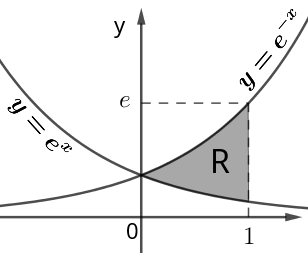
\includegraphics[width=0.37\textwidth]{figs/AreaEntcurvas/AreaEntCurvasExResol-e^xe^-x_2.png}
\label{e^x-e^-x}
}
%\caption{Representação de área limitada por curvas da forma $x=f(y)$ e $x=g(y)$}
\label{fig:Areas_y=4x-x^2_e^x-e^-x}
\end{figure}

\item Os gráficos das curvas cujas equações são \(y=e^x\), \(y=e^{-x}\) e a reta \(x=1\).

\begin{solution}
A região compreendida entre essas curvas é apresentada no item (b) da figura acima. Logo,

\[ \begin{array}{rcl} A_R= \mathlarger{\int}^{1}_{0} (e^x - e^{-x})\,dx &=& \left(e^x + e^{-x}\right)\Big{|}^{1}_{0} = (e +e^{-1}-2)^2. \end{array} \]
\end{solution}
\item A parábola \(y=-x^2 +4x-3\) e as retas tangentes a ela nos pontos \((0,-3)\) e \((3,0)\).

\begin{solution}
Observamos que \(y=-x^2 +4x-3 =1-(x-2)^2\) e, assim, a parábola \(y-1=-(x-2)^2\) tem vértice no ponto \((1,2)\). Além disso,

\(\dfrac{dy}{dx}\Big{|}_{x=3}= (-2x+4)\Big{|}_{x=3} =-2\), obtemos \(L_1: y-0=-2(x-3)\) de onde\\\\ \(L_1: 2x+y=6\);\\

\(\dfrac{dy}{dx}\Big{|}_{x=0}= (-2x+4)\Big{|}_{x=0} =4\), obtemos \(L_2: y+3=4(x-0)\) de onde\\\\ \(L_2: 4x-y=3\).

Assim, R está compreendida entre \(y=-x^2 +4x-3\), $L_1$ e \(L_2\) (veja o item (c) da figura abaixo). Logo,
\[ \begin{array}{rcl} A_R&=& \mathlarger{\int}^{3/2}_{0} \left[ (4x-3)-(-x^2+4x-3) \right]\,dx + \mathlarger{\int}^{3}_{3/2} \left[ (6-2x)-(-x^2+4x-3) \right]\,dx\\ &= &\mathlarger{\int}^{3/2}_{0} x^2 dx + \mathlarger{\int}^{3}_{3/2} (x^2-6x +9)dx \\ &=& \left(\dfrac{x^3}{3}\right)\Big{|}^{3/2}_{0} + \left( \dfrac{x^3}{3} -3x^2 +9x \right)\Big{|}^{3}_{3/2} =9+ \dfrac{27}{4}-\dfrac{27}{2} = \dfrac{9}{4} ^2. \end{array} \]
\end{solution}
\begin{figure}[H]
\centering
\subfigure[tesbte][]{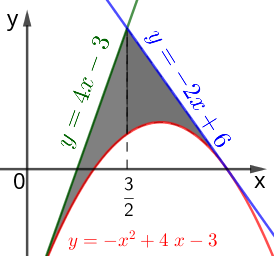
\includegraphics[width=0.36\textwidth]{figs/AreaEntcurvas/AreaEntreParab_4x-3_6-2x.png}
\label{-x^2+4x-3}
}
\qquad
\subfigure[cbb][]{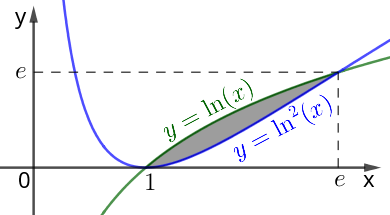
\includegraphics[width=0.42\textwidth]{figs/AreaEntcurvas/AreaEntrelnx-ln^2x.png}
\label{lnxln^2x}
}
%\caption{Representação de área limitada por curvas da forma $x=f(y)$ e $x=g(y)$}
\end{figure}
\item Os gráficos das funções \(y=\ln (x)\) e \(y=\ln^2( x)\).

\begin{solution}
Calculemos os pontos de interseção de ambas curvas:
\[ \left\{ \begin{array}{ccl} y&=& \ln(x)\\ y&=& \ln^2(x) \end{array} \right. \Rightarrow (\ln(x) )(\ln(x) -1) =0 \Rightarrow \ln(x) =0\,\,\mbox{ou}\,\,\ln(x) -1 =0 \Rightarrow \left\{ \begin{array}{ccl} x&=&e^0=1;\\ x&=&e^1. \end{array} \right. \]
Assim, R compreendida entre essas curvas é apresentada no item (d) da figura acima. Logo,
\[ \begin{array}{rcl} A_R &= &\mathlarger{\int}^{e}_{1} \left( \ln(x) -\ln^2(x) \right)dx \\ & = & \left( 3x\ln (x) -x\ln^2 (x) -3x \right)\Big{|}^{e}_{1} \\ & = & \left( 3(e)\ln (e) -(e)\ln^2 (e) -3e \right)-\left( 3(1)\ln (1) -(1)\ln^2 (1) -31 \right)\\ & = & (3-e) ^2. \end{array} \]
\end{solution}
\end{compactenum}
\end{exeresol}



\subsection{Exercícios}
\begin{exer}
Encontre a área da região sombreada.
\begin{multicols}{2}
\begin{description}
\item a) \\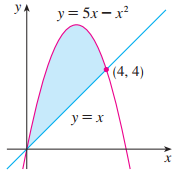
\includegraphics[scale=1.2]{figs/AreaEntcurvas/Area1Exer.png}\hfill 
 \item b)\\  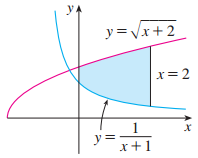
\includegraphics[scale=1.2]{figs/AreaEntcurvas/Area2Exer.png}
 \end{description}
\end{multicols}
\begin{multicols}{2}
\begin{description}
\item c)\\  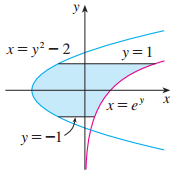
\includegraphics[scale=1.2]{figs/AreaEntcurvas/Area3Exer.png}
\item d)\\  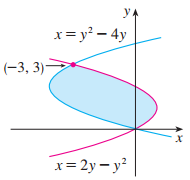
\includegraphics[scale=1.2]{figs/AreaEntcurvas/Area4Exer.png}
\end{description}
\end{multicols}
\end{exer}
\begin{exer}
Esboce a região delimitada pelas curvas indicadas e encontre sua área
\minipag{0.1}{}\hfill
\minipag{0.86}{
\begin{compactenum}[1. ]
\item $y = 12 - x^2, y = x^2 - 6$
\item $y = x^2, y = 4 x - x^2$
\item $y = e^x, y = xe^x, x = 0$
\item $x = 2 y^2, x = 4 + y^2$
\item $y=\sqrt{x-1}, x-y=1$
\item $x=y^4, y=\sqrt{2-x}, y=0$
\item $x=y^3, x=y$
\item $y=|x|, y=x^2-2$\\
\end{compactenum}
}%
\end{exer}
\begin{exer}
Encontre a área delimitada pelas curvas  $y = \cos x$ e $ y = 2 - \cos x$, em que $  0\leq x\leq   2\pi$
\end{exer}
\begin{exer}
Calcule a integral e interprete-a como a área de uma região. Esboce a região\\
\minipag{0.1}{}\hfill
\minipag{0.94}{a) $\intdef{0}{\pi/2}{|\sin x-\cos 2x|}$\hfill b) $\intdef{0}{4}{|\sqrt{x+2}-x|}$}
\end{exer}
\section{Volume de um Sólido de Revolução}
\begin{framed}
\begin{definition}
    Um \textbf{sólido de revolução} é o sólido obtido com a rotação (ou revolução) de uma região plana em torno de um eixo em seu plano. Esse eixo é denominado de \textbf{eixo de revolução}.
\end{definition}
\end{framed}
\begin{figure}[H]
    \centering
    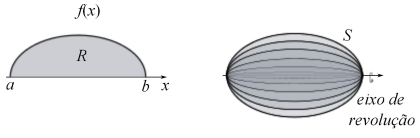
\includegraphics{figs/Volume/SolidoRevEixox.png}
    \caption{}
    %\label{fig:my_label}
\end{figure}
\begin{figure}[H]
    \centering
    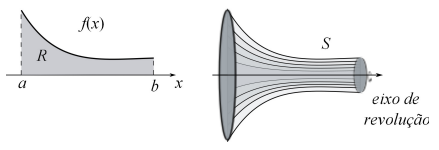
\includegraphics{figs/Volume/SolidoRevEixox2.png}
    \caption{}
 %   \label{fig:my_label}
\end{figure}

\subsection{Método do Disco Circular}
\subsubsection*{Caso I}
\begin{enumerate}[i.]
    \item Sejam \(f:[a,b] \to \mathbb{R}\) uma função contínua, e \(S\) o sólido de revolução obtido pela rotação em torno do eixo \(x\) da região plana \(R\) limitada pelo gráfico da curva \(y=f(x)\), pelo eixo \(x\) e pelas retas \(x=a\) e \(x=b\) (veja a figura acima). Assim, o volume de \(S\), denotado por \(V_S\) é dado por:

\[ V_S= \left( \pi \mathlarger{\int}^{b}_{a}\left[ f(x)\right]^2dx \right)\]
\item Sejam \(g:[c,d] \to \mathbb{R}\) uma função contínua, e \(S\) o sólido de revolução obtido pela rotação em torno do eixo \(y\) da região plana \(R\) limitada pela curva \(x=g(y)\), pelo eixo \(y\) e pelas retas \(y=c\) e \(y=d\). Assim, o volume de \(S\), denotado por \(V_S\) é dado por:

\[ V_S= \left( \pi \mathlarger{\int}^{d}_{c}\left[ g(y)\right]^2dy \right) \]
\end{enumerate}
\subsubsection*{Caso II}
\begin{enumerate}[i.]
    \item Sejam \(f, g:[a,b] \to \mathbb{R}\) duas funções contínuas cujos gráficos encontram-se ao mesmo lado do eixo \(x\). Além disso, \(|g(x)| \leq |f(x)|\), \(\forall\,x\in [a,b]\). Seja \(S\) o sólido de revolução obtido pela rotação em torno do eixo \(x\) da região \(R\) limitada pelas curvas \(y=f(x)\) e \(y=g(x)\), e pelas retas verticais \(x=a\), \(x=b\) (veja a figura a seguir). Assim, o volume de \(S\), denotado por \(V_S\) é dado por:

\[ V_S= \left( \pi \mathlarger{\int}^{b}_{a}\left( \left[ f(x)\right]^2 - \left[ g(x)\right]^2 \right)dx \right) \]
    \begin{figure}[H]
    \centering
    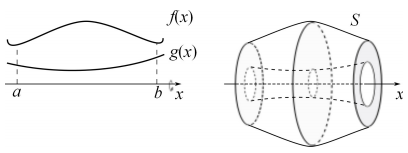
\includegraphics{figs/Volume/SolidoRevCaso2.png}
    \caption{}
   % \label{fig:my_label}
\end{figure}
\item Sejam \(f, g:[a,b] \to \mathbb{R}\) duas funções contínuas cujos gráficos encontram-se do mesmo lado da reta \(y=c\). Além disso, \(|g(x)-c| \leq |f(x)-c|\), \(\forall\,x\in [a,b]\). Seja \(S\) o sólido de revolução obtido pela rotação em torno da reta \(y=c\) da região \(R\) limitada pelas curvas \(y=f(x)\) e \(y=g(x)\) e pelas retas verticais \(x=a\) e \(x=b\). Assim, o volume de \(S\), denotado por \(V_S\) é dado por:

\[ V_S= \left( \pi \mathlarger{\int}^{b}_{a}\left( \left[ f(x)-c\right]^2 - \left[ g(x)-c\right]^2 \right)dx \right) \]
\item Sejam \(f, g:[a,b] \to \mathbb{R}\) duas funções contínuas cujos gráficos encontram-se do mesmo lado da reta \(x=k\). Além disso, \(|g(y)-k| \leq |f(y)-k|\), \(\forall\,y\in [c,d]\). Seja \(S\) o sólido de revolução obtido pela rotação em torno da reta \(x=k\) da região \(R\) limitada pelas curvas \(x=f(y)\) e \(x=g(y)\) e pelas retas horizontais \(y=c\) e \(y=d\). Assim, o volume de \(S\), denotado por \(V_S\) é dado por:

\[ V_S= \left( \pi \mathlarger{\int}^{d}_{c}\left( \left[ f(y)-k\right]^2 - \left[ g(y)-k\right]^2 \right)dy \right) \]
    \end{enumerate}
\begin{ex}
Calculemos o volume do sólido gerado pela rotação de R em torno:
\begin{compactenum}[a)]
\item do eixo \(x\), onde R é a região limitada pelos gráficos de \(y=e^x\), \(x=0\), \(x=1\) e \( y=0\).

\begin{solution}
A região R é apresentada no item (e) da figura a seguir. Aplicando o item (i) do Caso I, temos que:

\[ V_S= \pi \mathlarger{\int}^{1}_{0}\left( e^x\right)^2dx = \pi \mathlarger{\int}^{1}_{0} e^{2x} dx = \pi \left( \dfrac{e^{2x}}{2}\right) \Big{|}^{1}_{0} dx = \dfrac{\pi}{2} (e^2-1). \]

\begin{figure}[H]
\centering
\subfigure[itemda][]{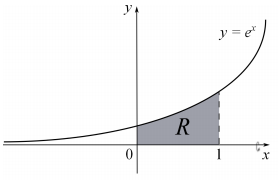
\includegraphics[width=0.45\textwidth]{figs/Volume/VolExerResolvR-e^x.png}}\qquad
\subfigure[itedmb][]{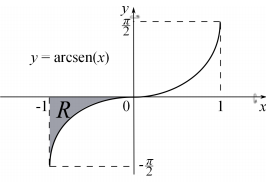
\includegraphics[width=0.45\textwidth]{figs/Volume/VolEntCurvasExResol-y=arcsenx.png}
%\label{XR-XL}
}
%\caption{Representação de área limitada por curvas da forma $x=f(y)$ e $x=g(y)$}
%\label{fig:Area-entre-curvas-x=fy-gy}
\end{figure}
\end{solution}
\item do eixo \(y\), onde R é a região limitada pelos gráficos de \(y={\rm arcsen}(x)\), \( x=-1\), \(y=0\) e \( y=-\pi/2\).

\begin{solution}
A região R é apresentada no item (f) da figura acima. Desde que o eixo de rotação é o eixo \(y\), consideramos \(y\) como a variável independente. Aplicando o item (iii) do Caso II, temos que:

\[ x=-1\,\,\, \Rightarrow \,\,\, f(y)=-1,\,\,\,y={\rm arcsen}(x)\,\,\, \Rightarrow \,\,\, x={\rm sen}(y)=g(y), \,\,\, c=-\dfrac{\pi}{2},\,\,\, d=0\,\,\, \mbox{e}\,\,\, k=0. \] Logo, \[ \begin{array}{rclcr} V_S= \pi \mathlarger{\int}^{0}_{-\pi/2}\left[ (-1)^2-({\rm sen}(y))^2\right]dy& =& \pi \mathlarger{\int}^{0}_{-\pi/2}\left[ 1-{\rm sen}^2(y)\right]dy \\ \\ &=& \pi \left[ \dfrac{y}{2} +\dfrac{1}{4}{\rm sen\,}(2y)\right]\Big{|}^{0}_{-\pi/2} = \dfrac{\pi}{4} \end{array} \]
\end{solution}
\item do eixo \(x\), onde R é a região limitada pelos gráficos de \(y=x^2\), \(y=\sqrt{x}\) e \( x=2\).

\begin{solution}
As curvas \(y=x^2\) e \(y=\sqrt{x}\) se intersectam nos pontos \((0,0)\) e \((1,1)\). A região R é apresentada no item (a) da figura abaixo, e podemos observar que \(x^2\leq \sqrt{x}\) para \(x\in[0,1]\), área representada por \(R_1\), e \(\sqrt{x} \leq x^2\) para \(x\in[1,2]\), área representada por \(R_2\). Aplicando o item (i) do Caso II para \(R_1\) e \(R_2\), temos que:

\[ \begin{array}{rcl} V_S &=& \pi \mathlarger{\int}^{1}_{0}\left[ (\sqrt{x})^2 -(x^2)^2\right]dx + \pi \mathlarger{\int}^{2}_{1}\left[ (x^2)^2 - (\sqrt{x})^2 \right]dx\\ & =& \pi \mathlarger{\int}^{1}_{0} (x-x^4)dx + \pi \mathlarger{\int}^{2}_{1} (x^4 -x)dx \\ &=& \pi\left(\dfrac{x^2}{2}-\pi\dfrac{x^5}{5}\right)\Big{|}^{1}_{0} + \left(\dfrac{x^5}{5}-\dfrac{x^2}{2}\right)\Big{|}^{2}_{2} \\ &=& \dfrac{3\pi}{10}+ \dfrac{47\pi}{10}=5\pi\,. \end{array} \]
\end{solution}
\begin{figure}[htb]
\center
\subfigure[itemc][]{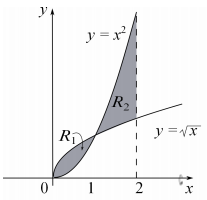
\includegraphics[width=0.43\linewidth]{figs/Volume/SolRevEx_x^2-sqrtx.png}
%\label{SolRev}
}\qquad
\subfigure[itemd][]{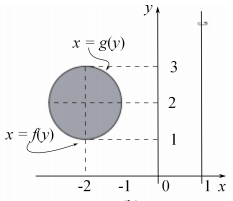
\includegraphics[width=0.45\linewidth]{figs/Volume/SolRevEx_x^2+y~2.png}
%\label{XR-XL}
}
%\caption{Representação de área limitada por curvas da forma $x=f(y)$ e $x=g(y)$}
\label{fig:VolumeSolREv}
\end{figure}
\item da reta \(x=1\), onde R é a região limitada pela circunferência \((x+2)^2+(y-2)^2=1\).

\begin{solution}
A região R é apresentada no item (b) da figura acima, e podemos observar que \(f(y)= -2 -\sqrt{1-(y-2)^2}\) e \(g(y)= -2 +\sqrt{1-(y-2)^2}\) verificando que \(1-g(y) \leq 1-f(y)\), \(c=1\) e \(d=3\). Aplicando o item (iii) do Caso II, temos que:

\[ \begin{array}{rcl} V_S &=& \pi \mathlarger{\int}^{3}_{1}\left[ (1-f(y))^2 -(1-g(y))^2\right]dy \\ &=& \pi \mathlarger{\int}^{3}_{1}\left[ \left(3+\sqrt{1-(y-2)^2}\right)^2 -\left(3-\sqrt{1-(y-2)^2}\right)^2\right]dy \\ &=& \pi \mathlarger{\int}^{3}_{1} 6\left(2\sqrt{1-(y-2)^2}\right)dy \\ &=& 12\pi \mathlarger{\int}^{3}_{1} \sqrt{1-(y-2)^2}\,dy \\ &=& 6 \pi\left[ (y-2)\sqrt{1-(y-2)^2} + {\rm arcsen}(y-2)\right]\Big{|}^{3}_{1}= 10\pi^2\,. \end{array} \]
\end{solution}
\end{compactenum}
\end{ex}
\subsection{Método das Cascas Cilíndricas}
\subsubsection* {Caso I}
Sejam \(a\geq 0\), \(f:[a,b] \to \mathbb{R}\) uma função contínua e não negativa, e \(S\) o sólido de revolução obtido pela rotação em torno do eixo \(y\) da região plana \(R\) limitada pelo gráfico da curva \(y=f(x)\), pelo eixo \(x\) e pelas retas \(x=a\) e \(x=b\) (veja a figura a seguir). Então, o volume de \(S\), denotado por \(V_S\), é dado por:
\begin{equation}
    V_S=   \int^{b}_{a}\, 2\pi x\,f(x)\,dx \label{eq:VolMetCascasForm1}
\end{equation}
\begin{figure}[H]
    \centering
    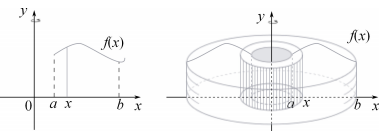
\includegraphics{figs/Volume/VolSolCascascilindricas.png}
    \caption{}
   % \label{fig:my_label}
\end{figure}

A melhor maneira de lembrar a Fórmula \eqref{eq:VolMetCascasForm1} é pensar em uma concha típica, cortada e achatada como na Figura \ref{fig:ExplicandoVolCascas}, com raio $x$, circunferência $2\pi x$, altura $f(x)$ e espessura $\Delta x$ ou $dx$:
\[\int_a^b \underbrace{(2\pi x)}_{\text{Circunferência}}\qquad\underbrace{f(x)]}_{\text{altura}}\quad \underbrace{dx}_{\text{espessura}}\]
\begin{figure}[htb]
    \centering
    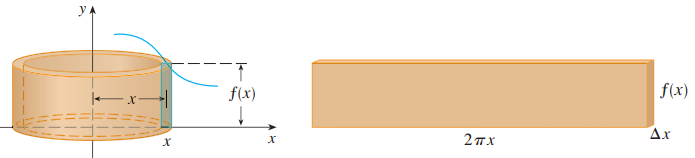
\includegraphics[width=\textwidth]{figs/Volume/ExplicForm-2pixfx.png}
    \caption{}
    \label{fig:ExplicandoVolCascas}
\end{figure}
Esse tipo de argumento será útil em outras situações, tais como quando giramos em torno
de outras retas além do eixo $y$.
\subsubsection*{Caso II}
Sejam \(f,g:[a,b] \to \mathbb{R}\) duas funções contínuas em \([a,b]\) tais que \(g(x)\leq f(x)\), \(\forall\, x\in [a,b]\). Seja \(R\) a região limitada pelas curvas \(y=f(x)\) e \(y=g(x)\), e pelas retas \(x=a\) e \(x=b\). Dado \(c \notin (a,b)\), temos que:
\begin{enumerate}[i.]
    \item se \(c\leq a\), então o volume do sólido de revolução \(S\) obtido pela rotação de R em torno da reta \(x=c\) (veja o item (a) da figura a seguir) é dado por:

\[ V_S= \left( 2\pi \mathlarger{\int}^{b}_{a} (x-c)\left[f(x)-g(x)\right]\,dx \right); \]
\begin{figure}[H]
\center
\subfigure[a][]{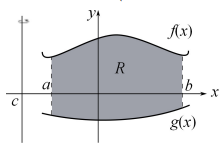
\includegraphics[width=0.43\textwidth]{figs/Volume/VolCascasf-g.png}
%\label{SolRev}
}\qquad
\subfigure[c][]{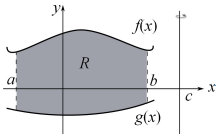
\includegraphics[width=0.45\textwidth]{figs/Volume/VolCascasf-g2.png}
%\label{XR-XL}
}
%\caption{Representação de área limitada por curvas da forma $x=f(y)$ e $x=g(y)$}
%\label{fig:Area-entre-curvas-x=fy-gy}
\end{figure}
\item se \(b\leq c\), então o volume do sólido de revolução \(S\) obtido pela rotação de R em torno da reta \(x=c\) (veja o item (b) da figura acima) é dado por:

\[ V_S= \left( 2\pi \mathlarger{\int}^{b}_{a} (c-x)\left[f(x)-g(x)\right]\,dx \right). \]
\end{enumerate}
\nota{
Sejam \(f\) e \(g\) duas funções contínuas em \([a,b]\) tais que \(g(y)\leq f(y)\), \(\forall\, y\in [a,b]\). Seja \(R\) a região limitada pelas curvas \(x=f(y)\) e \(x=g(y)\), e pelas retas \(y=a\) e \(y=b\). Dado \(c \notin (a,b)\), temos que:
\begin{compactenum}[i.]
\item se \(c\leq a\), então o volume do sólido de revolução \(S\) obtido ao rotar R em torno da reta \(y=c\) é dado por:
\[ V= \left( 2\pi \mathlarger{\int}^{b}_{a} (y-c)\left[f(y)-g(y)\right]\,dy \right)\]
\item se \(b\leq c\), então o volume do sólido de revolução \(S\) obtido ao rotar R em torno da reta \(y=c\) é dado por:
\[ V= \left( 2\pi \mathlarger{\int}^{b}_{a} (c-y)\left[f(y)-g(y)\right]\,dy \right) \]
\end{compactenum}
}
\begin{ex}
Encontre o volume do sólido obtido por rotação  em torno do eixo da região delimitada por: $y=2x^2-x^3$ e $x=0$.

\begin{solution}

\pichskip{0.2cm}%distância entre texto e figura
\parpic[r]{%\includegraphics[scale=0.75]{cap_apl_integracao/figs/Volume/AreaEntreFuncSenCos.png}}
\begin{minipage}{0.45\textwidth}
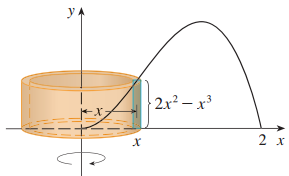
\includegraphics[scale=0.85]{figs/Volume/ExIlustradoVolCascas.png}
\captionof{figure}{}%
\label{fig:ExIlustrativoVolCascas}
\end{minipage}
}
\noindent A partir do esboço da Figura \ref{fig:ExIlustrativoVolCascas} ao lado vemos que uma concha típica tem raio $x$, circunferência $2\pi x$ e altura $f(x)=2x^2-x^3$. Então, o volume é
\begin{align*}
    V_S&=\int_0^2 (2\pi x) (2x^2-x^3) dx\\
    &=2\pi\intdef{0}{2}{(2x^3-x^4)}\\
    &=2\pi\pr{\frac{1}{2}x^4-\frac{1}{5}x^5}_0^2=2\pi\pc{8-\frac{32}{5}}=\frac{16}{5}\pi
\end{align*}
\end{solution}
\end{ex}

\begin{ex}~
\begin{compactenum}[a)]
\item Calculemos o volume do sólido obtido ao rotar R em torno do eixo \(y\), onde R é a região limitada pela curva \(y=(x-2)^3\), pelo eixo \(x\) e pela reta \(x=3\).

\begin{solution}
R é apresentada no item (a) da figura abaixo. Nesse caso, aplicamos o Caso I e o volume é dado por:

\[\begin{array}{rcl} V_S&=& 2\pi \mathlarger{\int}^{3}_{2}x\,f(x)\,dx = 2\pi \mathlarger{\int}^{3}_{2}x(x-2)^3dx= 2\pi \mathlarger{\int}^{3}_{2}(x^4-6x^3+12x^2-8x)dx\\ \\ &=& 2\pi \left(\dfrac{x^5}{5}-\dfrac{3x^4}{2}+4x^3-4x^2\right)\Big{|}^{3}_{2} = \dfrac{14\pi}{10}. \end{array} \]
\end{solution}
\begin{figure}[H]
\centering
\subfigure[\label{a}][]{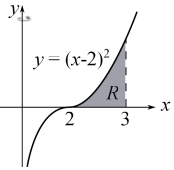
\includegraphics[width=0.32\linewidth]{figs/Volume/SolRevCascasEx-a.png}
%\label{SolRev}
}\hfill
\subfigure[b][]{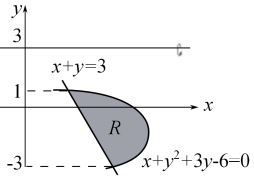
\includegraphics[width=0.32\linewidth]{figs/Volume/SolRevCascasEx-b.png}
%\label{XR-XL}
}\hfill
\subfigure[cc][]{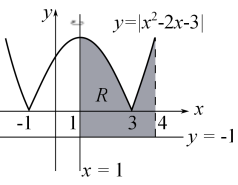
\includegraphics[width=0.32\linewidth]{figs/Volume/SolRevCascasEx-c.png}
%\label{XR-XL}
}
%\caption{Representação de área limitada por curvas da forma $x=f(y)$ e $x=g(y)$}
%\label{fig:Area-entre-curvas-x=fy-gy}
\end{figure}
\item Calculemos o volume do sólido obtido na rotação da região limitada pelos gráficos de \(x+y^2+3y-6=0\), \(x+y-3=0\), em torno da reta \(y=3\).

\begin{solution}
R é apresentada no item (b) da figura acima, e desde que o eixo de revolução é horizontal, nesse caso, aplicamos o item (ii) da Nota acima, para \(c=3\). Logo, o volume é dado por:
\[\begin{array}{rcl} V_S&=& 2\pi \mathlarger{\int}^{1}_{-3}(3-y)\left[(6-3y-y^2)-(3-y) \right]\,dy =2\pi \mathlarger{\int}^{1}_{-3}(y^3-y^2-9y+9)dy\\ \\ &=& 2\pi \left(\dfrac{y^4}{4}-\dfrac{y^3}{3}-\dfrac{9y^2}{2}+9y\right)\Big{|}^{1}_{-3} = \dfrac{256\pi}{3}. \end{array} \]
\end{solution}
\item Calculemos o volume do sólido de revolução obtido na rotação da região limitada pelos gráficos de \(y=|x^2-2x-3|\), \(y+1=0\), \(x-1=0\) e \(x-4=0\), em torno da reta \(x=1\).

\begin{solution}
Notemos que:

\[ |x^2-2x-3|= |(x-3)(x+1)|=\left\{ \begin{array}{ccl} -(x^2-2x-3),& & 1\leq x< 3;\\ x^2-2x-3,& & 3\leq x\leq 4. \end{array} \right. \]
R é a região apresentada no item (c) da figura acima e, nesse caso, aplicamos o item (i) do Caso II, para \(c=1\). Logo, o volume é dado por:

\[ \begin{array}{rcl} V_S &=& 2\pi \mathlarger{\int}^{4}_{1}(x-1)\left[|x^2-2x-3|-(-1) \right]\,dx\\ &=& 2\pi \left(\mathlarger{\int}^{3}_{1} (x-1)\left[(3+2x -x^2)+1 \right]\,dx + \mathlarger{\int}^{4}_{3}(x-1)\left[(x^2-2x-3)+1 \right]\,dx\right)\\ &=& 2\pi \left( \mathlarger{\int}^{3}_{1}\left(-4+2x+3x^2-x^3 \right)\,dx + \mathlarger{\int}^{4}_{3}\left(x^3 -3x^2+2\right)\,dx \right)\\ &=& 2\pi \left( \left(-4x+x^2+x^3-\frac{x^4}{4} \right)\Big{|}^{3}_{1} + \left(\dfrac{x^4}{4} -x^3+2x\right)\Big{|}^{4}_{3} \right)\\ &=& 2\pi \left( 6+\dfrac{35}{4} \right)= \dfrac{59}{2}\pi\, \end{array} \]
\end{solution}
\end{compactenum}
\end{ex}

\section{Comprimento de arcos}\index{curvas}\index{Arcos!comprimento}
\subsection*{Comprimento de uma curva $y = f(x)$}
Consideremos uma função \(f:[a,b] \to \mathbb{R}\) com derivada contínua no intervalo \([a,b]\) e uma partição \(P=\{x_0,x_1,\ldots,x_n \}\) do intervalo \([a,b]\). P define uma poligonal formada pelos segmentos retilíneos a partir do ponto \(P_{i-1}(x_{i-1},f(x_{i-1}))\) até o ponto \(P_i=(x_{i},f(x_{i}))\), para \(i=1,2,\dots,n\).
\begin{figure}
    \centering
    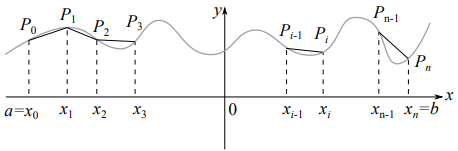
\includegraphics{figs/CompArcos/IlustCompArcos.png}
    \caption{}
    \label{fig:IlustCompArcos}
\end{figure}
O comprimento do i-ésimo segmento definido pela partição \(P\) é:

\[ \left|\overline{P_{i-1}P_i} \right|=\sqrt{(x_i - x_{i-1})^2 + (f(x_i) - f(x_{i-1}))^2 }. \]
Portanto, o comprimento da poligonal definida pela partição \(P\) é:

\[ L_P = \sum\limits^{n}_{i=1}\left|\overline{P_{i-1}P_i} \right|=\sum\limits^{n}_{i=1}\sqrt{(x_i - x_{i-1})^2 + (f(x_i) - f(x_{i-1}))^2 }. \]

\begin{framed}
\begin{definition}
    Seja \(f:[a,b] \to \mathbb{R}\) uma função com derivada contínua em \([a,b]\). Se existe um número \(L\) tal que

\[ L= \lim\limits_{\|P\|\to 0} \sum\limits^{n}_{i=1}\left|\overline{P_{i-1}P_i} \right|, \]
então diz-se que o arco \(P_0 P_n\) da curva \(y=f(x)\) é retificável e \(L\) é o comprimento de arco da curva \(y=f(x)\) a partir do ponto \(P_0=(a,f(a))\) até o ponto \(P_n=(b,f(b))\).
\end{definition}
\end{framed}
\begin{framed}
\begin{teo}
Seja \(f:[a,b] \to \mathbb{R}\) uma função com derivada contínua em \([a,b]\). Então, o comprimento de arco da curva \(y=f(x)\) a partir do ponto \((a,f(a))\) até \((b,f(b))\) é dado por:

\[ L=\mathlarger{\int}^{b}_{a} \sqrt{ 1+ \left(f'(x)\right)^2} dx= \mathlarger{\int}^{b}_{a} \sqrt{ 1+ \left(\dfrac{dy}{dx}\right)^2} dx \]
\end{teo}
\end{framed}
\nota{
Se \(g:[c,d] \to \mathbb{R}\) é uma função contínua em \([c,d]\), então o comprimento de arco da curva \(x=g(y)\) a partir do ponto \((g(c),c)\) até \((g(d),d)\) é dado por:

\[ L= \mathlarger{\int}^{d}_{c} \sqrt{ 1+ \left(g'(y)\right)^2} dy=\mathlarger{\int}^{d}_{c} \sqrt{ 1+ \left(\dfrac{dx}{dy}\right)^2} dy \]
\begin{center}
    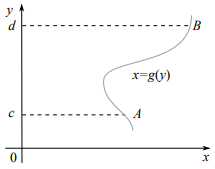
\includegraphics{figs/CompArcos/CompCurvaDiry.png}
\end{center}
}
\begin{ex}
Encontremos o comprimento de arco:
\begin{compactenum}[a)]
\item da parábola \(6y=x^2\), desde a origem de coordenadas até o ponto \(\left(4,\dfrac{8}{3}\right)\).

\begin{solution}
Como \(6y=x^2\) (veja o item (a) da figura a seguir) então \[\dfrac{dy}{dx}=\dfrac{x}{3}\] Logo,

\[ \begin{array}{rcl} L&=& \mathlarger{\int}^{4}_{0} \sqrt{ 1+ \left(\dfrac{dy}{dx}\right)^2} dx = \mathlarger{\int}^{4}_{0} \sqrt{ 1+ \dfrac{x^2}{9}} dx= \dfrac{1}{3} \mathlarger{\int}^{4}_{0} \sqrt{9+x^2}\, dx\\ \\ &=&\dfrac{1}{3}\left[ \dfrac{x}{2}\sqrt{9-x^2} + \dfrac{9}{2}\ln\left|x+\sqrt{x^2+9} \right| \right]\Big{|}^{4}_{0}\,\,=\,\,\dfrac{1}{3}\left[ \left( 10+\dfrac{9}{2} \ln 9 \right) - \left( 0+\dfrac{9}{2} \ln 3 \right) \right]\\ \\ &=&\dfrac{1}{3} \left[ 10+\dfrac{9}{2} \ln (3) \right]. \end{array} \]
\end{solution}\vspace{-0.5cm}
\begin{figure}[H]
\centering
\subfigure[\label{a}][]{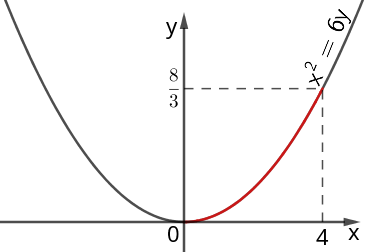
\includegraphics[width=0.45\linewidth]{figs/CompArcos/CompArcoParab.png}
%\label{SolRev}
}\quad
\subfigure[b][]{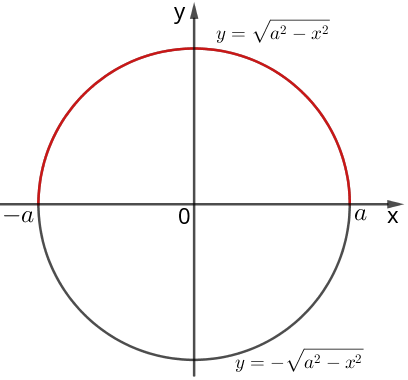
\includegraphics[width=0.42\linewidth]{figs/CompArcos/CompArco-SemiCircEx.png}
%\label{XR-XL}
}
%\caption{Representação de área limitada por curvas da forma $x=f(y)$ e $x=g(y)$}
%\label{fig:Area-entre-curvas-x=fy-gy}
\end{figure}
\item da circunferência \(x^2+y^2 =a^2\).

\begin{solution}

Da equação \(x^2+y^2 =a^2\), obtemos \(y=\pm \sqrt{a^2-x^2}\) (veja o item (b) da figura acima).\\ Além disso, observamos que o gráfico é simétrico com respeito do eixo \(x\). Então, podemos considerar \(y=\sqrt{a^2-x^2}\) o que implica que \[\dfrac{dy}{dx}=\dfrac{-x}{\sqrt{a^2-x^2}}\].\\ Portanto, o comprimento de arco é:

\[ \begin{array}{rcl} L&=& 2\mathlarger{\int}^{a}_{-a} \sqrt{ 1+ \left(\dfrac{dy}{dx}\right)^2} dx = 2\mathlarger{\int}^{a}_{-a} \sqrt{ 1+ \dfrac{x^2}{a^2-x^2}} dx= 2a \mathlarger{\int}^{a}_{-a} \dfrac{1}{\sqrt{a^2-x^2}} dx \\ \\ &=& 2a\, {\rm arcsen}\left(\dfrac{x}{a}\right) \Big{|}^{a}_{-a} = 2a\left( {\rm arcsen\,}(1) - {\rm arcsen\,}( -1) \right) \\ \\ &=&2a \left( \dfrac{\pi}{2} - \left(-\dfrac{\pi}{2} \right)\right) = 2a \pi \end{array} \]
\end{solution}
\item total da curva \( x^{2/3} + y^{2/3} = a^{2/3}\).

\begin{solution}
Da equação \(x^{2/3} + y^{2/3} = a^{2/3}\), obtemos que \(y = \left( a^{2/3} -x^{2/3} \right)^{3/2}\) e \(\dfrac{dy}{dx}=-x^{-1/3} \sqrt{a^{2/3} -x^{2/3} }\). Além disso, o gráfico da curva é simétrico com respeito à origem (veja o item (a) da figura abaixo). Logo, temos que:

\[ \begin{array}{rcl} L&=& 4\mathlarger{\int}^{a}_{0} \sqrt{ 1+ \left(\dfrac{dy}{dx}\right)^2} dx = 4 \mathlarger{\int}^{a}_{0} \sqrt{ 1+ x^{-2/3}\left(a^{2/3} -x^{2/3} \right)} dx \\ \\ &=& 4 \mathlarger{\int}^{a}_{0} \sqrt{ a^{2/3} x^{-2/3}} dx = 4a^{1/3} \mathlarger{\int}^{a}_{0} x^{-1/3} dx = 6 a^{1/3}x^{2/3} \Big{|}^{a}_{0}=6a\end{array} \]
\end{solution}
\begin{figure}[H]
\centering
\subfigure[\label{a}][]{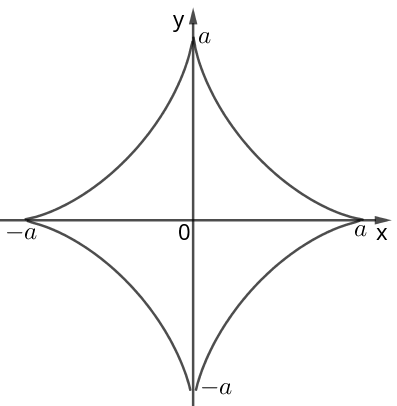
\includegraphics[width=0.42\linewidth]{figs/CompArcos/CompArco_-a_a.png}
%\label{SolRev}
}\quad
\subfigure[b][]{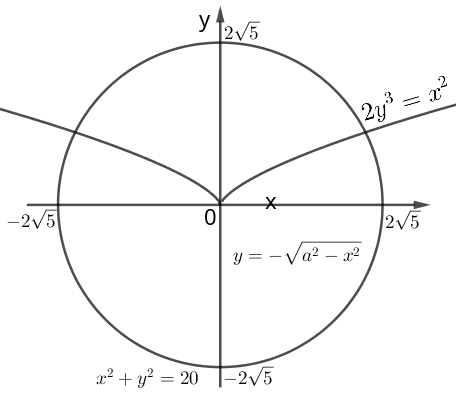
\includegraphics[width=0.45\linewidth]{figs/CompArcos/CompArcoEx-x^2+y^2=20.png}
%\label{XR-XL}
}
%\caption{Representação de área limitada por curvas da forma $x=f(y)$ e $x=g(y)$}
%\label{fig:Area-entre-curvas-x=fy-gy}
\end{figure}
\item da parábola semicúbica \(2y^3=x^2\) no interior da circunferência \(x^2+y^2=20\).

\begin{solution}
Os pontos de interseção de ambas curvas são \((-4,2)\) e \((4,2)\). Ao derivar a equação \(2y^3=x^2\) implicitamente com respeito a variável \(y\), temos que:

\[ \dfrac{dx}{dy}= \dfrac{3y^2}{x}\,\Rightarrow\,1+\left( \dfrac{dx}{dy}\right)^2 = 1+\dfrac{9y^4}{x^2}=1+9y \left(\dfrac{y^3}{x^2} \right) = 1+ \dfrac{9y}{2}. \]
Além disso, o gráfico é simétrico em relação ao eixo \(y\) (veja o item (b) da figura acima). Logo,

\[ \begin{array}{rcl} L= 2\mathlarger{\int}^{2}_{0} \sqrt{ 1+ \left(\dfrac{dx}{dy}\right)^2} dx &= & 2\mathlarger{\int}^{2}_{0} \sqrt{ 1+ \dfrac{9y}{2}} dy \\ \\ &=& 2 \left(\dfrac{4}{27} \left(1+ \dfrac{9y}{2}\right)^{3/2} \right)\Big{|}^{2}_{0}=\dfrac{8}{27}\left(10\sqrt{10}-1 \right) \end{array} \]
\end{solution}
\end{compactenum}
\end{ex}
\section{Área de uma Superfície de Revolução}   
Seja \(f:[a,b] \to \mathbb{R}\) uma função não negativa e com derivada contínua no intervalo \([a,b]\). Ao girar o gráfico de \(f\) de \(x=a\) até \(x=b\), em torno do eixo \(x\) é obtida uma superfície de revolução (veja a figura abaixo). A área dessa superfície de revolução, denotada por \(A_S\), é dada por:

\[ A_S=\left( 2\pi \mathlarger{\int}^{b}_{a} f(x)\,\sqrt{ 1+ \left(f'(x)\right)^2} dx\right) \mbox{ unidades}^2. \]
\begin{figure}[H]
    \centering
    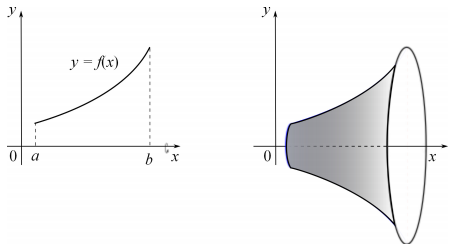
\includegraphics{figs/SupRev/SupRev.png}
    \vspace{-0.5cm}
   \caption{}
    \label{fig:SupRev}
\end{figure}
\nota{
\begin{compactenum}[a.]
\item Seja \(f:[a,b] \to \mathbb{R}\) uma função com derivada contínua no intervalo \([a,b]\), é possível encontrar seu gráfico do mesmo lado da reta \(y=c\). Ao girar o gráfico de \(f\) a partir de \(x=a\) até \(x=b\), em torno da reta \(y=c\), obtemos uma superfície de revolução cuja área é:

\[ A_S=\left( 2\pi \mathlarger{\int}^{b}_{a} |f(x)-c|\,\sqrt{ 1+ \left(f'(x)\right)^2} dx\right) \mbox{ unidades}^2. \]
\item Se \(x=g(y)\) é uma função com derivada contínua no intervalo \([a,b]\), encontraremos seu gráfico do mesmo lado da reta \(x=c\). Ao girar o gráfico de \(g\), a partir de \(y=a\) até \(y=b\), em torno da reta \(x=c\), obteremos uma superfície de revolução cuja área é:

\[ A_S=\left( 2\pi \mathlarger{\int}^{b}_{a} |g(y)-c|\,\sqrt{ 1+ \left(g'(y)\right)^2} dy\right) \mbox{ unidades}^2. \]
\end{compactenum}
}
\begin{ex}
Calculemos a área da superfície gerada ao girar:
\begin{compactenum}[a)]
\item o gráfico de \(f(x)=\sqrt{24-4x}\), \(x\in[3,6]\), em torno do eixo \(x\).

\begin{solution}
Ao derivar \(f\) temos que \(f'(x)=\dfrac{-2}{\sqrt{24-4x}}\), e a área da superfície é:

\[ \begin{array}{rcl} A_S&=& 2\pi \mathlarger{\int}^{6}_{3} f(x)\,\sqrt{ 1+ \left(f'(x)\right)^2} dx\,\,=\,\, 2\pi \mathlarger{\int}^{6}_{3}\sqrt{24-4x} \sqrt{ 1+ \dfrac{4}{24-4x}}\, dx\\ \\ & =& 2\pi \mathlarger{\int}^{6}_{3} \sqrt{28-4x}\, dx =2\pi\left(-\dfrac{1}{6}\left(28-4x\right)^{3/2}\right)\Big{|}^{6}_{3}=\dfrac{56\pi}{3} \mbox{ unidades}^2. \end{array} \]
\end{solution}
\begin{figure}[H]
\centering
\subfigure[\label{a}][]{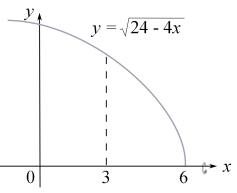
\includegraphics[width=0.3\textwidth]{figs/SupRev/SupRevExa.png}
%\label{SolRev}
}\hfill
\subfigure[b][]{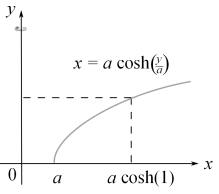
\includegraphics[width=0.3\textwidth]{figs/SupRev/SupRevExb.png}
%\label{XR-XL}
}\hfill 
\subfigure[b][]{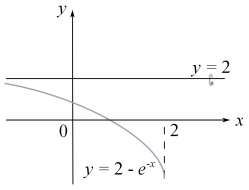
\includegraphics[width=0.3\textwidth]{figs/SupRev/SupRevExc.png}
%\label{XR-XL}
}
%\caption{Representação de área limitada por curvas da forma $x=f(y)$ e $x=g(y)$}
%\label{fig:Area-entre-curvas-x=fy-gy}
\end{figure}
\item o gráfico da curva \(y=a \cosh^{-1}\left(\dfrac{x}{a}\right)\), a partir de \(x=a\) até \(a\cosh( 1)\), em torno do eixo \(y\).

\begin{solution}
Considerando \(x=f(y)=a \cosh\left(\dfrac{y}{a}\right)\), obtemos \(\dfrac{dx}{dy}=f'(y)= {\rm senh} \left(\dfrac{y}{a}\right)\). Além disso, como a curva gira em torno do eixo \(y\), a área da superfície gerada é:

\[ \begin{array}{rcl} A_S&=& 2\pi \mathlarger{\int}^{a}_{0} f(y)\,\sqrt{ 1+ \left(f'(y)\right)^2} dy= 2\pi \mathlarger{\int}^{a}_{0} a \cosh\left(\dfrac{y}{a}\right) \,\sqrt{ 1+ {\rm senh}^2 \left(\dfrac{y}{a}\right)} dy\\ &=& 2\pi \mathlarger{\int}^{a}_{0} a \cosh^2\left(\dfrac{y}{a}\right) dy = \pi a \mathlarger{\int}^{a}_{0} \left(\cosh\left(\dfrac{2y}{a}\right)+ 1 \right) dy \\ \\ &=& \pi a \left(\dfrac{a}{2} {\rm senh}\left(\dfrac{2y}{a}\right)+ y\right) \Big{|}^a_0=\dfrac{\pi a^2}{2}(2+{\rm senh}\,2)\mbox{ unidades}^2. \end{array} \]
\end{solution}
\item a curva \(y=2-e^x\), a partir de \(x=0\) até \(c=2\), em torno da reta \(y=2\).

\begin{solution}
Da equação \(y=2-e^x\), obtemos \(\dfrac{dy}{dx}=f'(x)=-e^x\), assim, a área da superfície é:

\[ \begin{array}{rcl} A_S &=& 2\pi \mathlarger{\int}^{2}_{0} (2-f(x))\sqrt{ 1+ \left(f'(x)\right)^2} dx = 2\pi \mathlarger{\int}^{2}_{0} e^x\sqrt{ 1+ (e^x)^2} dx \end{array} \] Fazendo $z=e^x$ temos que $dz=e^x\,dx$, $x=2$ implica $z=e^2$ e $x=0$ implica $z=e^0=1$. Assim \[ \begin{array}{rcl} 2\pi \mathlarger{\int}^{2}_{0} e^x\sqrt{ 1+ (e^x)^2} dx &=& 2\pi \mathlarger{\int}^{e^2}_{1} \sqrt{ 1+ z^2} dz \\ \\ &=& 2\pi \left[ \dfrac{1}{2} \left(z\sqrt{1+z^2} + \ln \left( z+\sqrt{1+z^2} \right) \right) \right] \Big{|}^{e^2}_{1} \end{array} \] Portanto, \[ \begin{array}{rcl} A_S&=&\pi \left[ e^2\sqrt{1+e^4} -\sqrt{2} + \ln \left( \dfrac{e^2+\sqrt{1+e^4}}{1+\sqrt{2}} \right) \right] \mbox{ unidades}^2 \end{array} \]
\end{solution}
\end{compactenum}
\end{ex}

 

\section{Aplicações na Física}\index{Aplicações!Física}\label{AplicFisica}
\subsection{Trabalho}\index{Aplicações!trabalho}\label{subsec:AplicTrabalho}
No caso de uma força constante F, o trabalho realizado é definido pelo produto da força pela distância d que o objeto se move:
\begin{center}
    $\tau=Fd\hspace{2cm}\text{ trabalho}=\text{força} \times \text{distância}$
\end{center}

Consideremos o deslocamento da partícula de $x = a$ até $x = b$ com \(a < b\) e suponhamos que \(F(x) \) seja
contínua no intervalo \([a,b]\). Seja \(P = (x_i)\) uma partição do intervalo \([a,b]\) e escolhemos \(x_i^*\in [x_{i-1}, x_i],  i = 1, \ldots,n\).

Se \(\Delta x_i = x_i -x_{i-1}\) for suficientemente pequeno, $F$ será praticamente constante no intervalo, e então podemos dizer que trabalho realizado pela força de \(x_{i-1}\) até \(x_i \) será
aproximadamente
$$\tau_i=F(x_i^*)\Delta x_i$$
Logo podemos aproximar o trabalho realizado por \(F\) de \(a\) até \( b\) pela soma dos trabalhos realizados nos intervalos $[x_{i-1}, x_i],  i = 1, \ldots ,n$, isto é
\[\tau=\sum_{i=1}^n  F(x_i^*)\Delta x_i\]
A intuição acima nos motiva a definirmos trabalho como:
\begin{framed}
\begin{definition}
    O trabalho $\tau$ realizado por uma força $F$ sobre uma partícula
no deslocamento de $x = a$ até $x = b$ é dado por
\[\tau=\lim_{\Delta x\to 0} \sum_{i=1}^n  F(x_i^*)\Delta x_i=\int_a^b F(x) dx\]
\end{definition}
\end{framed}
\hrule
\begin{ex}
Sobre uma partícula que se desloca sobre o eixo $x|$ atua uma força paralela ao deslocamento e de componente $f(x)=\frac{1}{x^2}$. Calcule o trabalho realizado pela força no deslocamento de $x = 1$ até $x = 2$.\\
\begin{solut}
$$\tau=\intdef{1}{2}{\frac{1}{x^2}}=\left.-\frac{1}{x}\right]_1^2=\frac{1}{2}$$
\end{solut}
\end{ex}
\begin{ex}
Considere uma mola sobre uma superfície horizontal com uma das extremidades fixa num anteparo. Suponha que a origem \(x = 0\) coincide com a extremidade livre quando a mola não está comprimida nem distendida. Agora, suponha que a mola seja distendida e que uma partícula seja presa à sua extremidade livre. Considere que a força exercida sobre a mola obedece a Lei de Hooke: \(F(x) = -kx\), onde \(k\) é a constante elástica da mola. Calcule o trabalho realizado pela mola quando a partícula se desloca das posições \(x = 0,5\) até
\(x = 0 \) e \(x = 0,5\) até \(x = -0,5\).\\
\begin{solut}
O trabalho realizado pela mola quando a partícula se desloca de  \(x = 0,5\) até
\(x = 0 \) é:
\matt{
\tau=\intdef{1/2}{0}{-kx}=\left.-k\frac{x^2}{2}\right|_{1/2}^0=\frac{k}{8}
}

Já o trabalho realizado pela mola quando a partícula se desloca de  \(x = 0,5\) até
\(x = -0.5 \) é dado por:
\matt{
\tau=\intdef{1/2}{-1/2}{-kx}=\left.-k\frac{x^2}{2}\right|_{1/2}^{-1/2}=0
}
\end{solut}
\end{ex}
\subsection{Fórmulas do MRU e MRUV}
Você conhece da física a fórmula da posição do Movimento Retilíneo Uniforme - MRU dada por $s=s_0+vt$, onde a aceleração é nula e por conta disso a velocidade é constante. Também conhece as fórmulas da posição e velocidade do Movimento Uniformemente Variado - MRUV, onde a aceleração é constante, as quais são: $V=V_0+at$ (Fórmula da velocidade) e $S=S_0+v_0t+\frac{a}{2}t^2$ (Fórmula da posição) que nada mais são que funções matemáticas de primeiro e segundo graus (função afim e quadrática, respectivamente).

Nesta seção, a partir da definição de aceleração como a derivada da velocidade em relação ao tempo, ou seja, $a=\frac{dv}{dt}$ e, a velocidade como a derivada da posição em relação ao tempo, isto é, $v=\frac{ds}{dt}$, deduzir as fórmulas do MRUV acima.
\subsubsection*{Obtendo a fórmula da velocidade}
Sabendo que $a=\frac{dv}{dt}$ seque que
\begin{equation}
    v(t)=\int a\, dt=at+C\label{eq:acel-to-veloc}
\end{equation}
Suponhamos que uma partícula se desloca ao longo de uma linha reta com velocidade inicial $v(t_0)=v_0$,  sendo $t_0=0$ o instante inicial. Assim iremos obter a fórmula que permite calcular sua velocidade em qualquer instante $t$, substituindo $t=0$ e $v(t_0)=v_0$ na equação \eqref{eq:acel-to-veloc}, temos $v_0=a*0+C\Rightarrow C=v_0$, voltando a equação \eqref{eq:acel-to-veloc}, temos que 
\begin{equation}
 \boldsymbol{ v(t)=v_0+at  }
\end{equation}

\subsubsection*{Obtendo a fórmula da posição}
Analogamente, sabendo que $v=\frac{ds}{dt}$ seque que
\begin{equation}
    s(t)=\int v\, dt=\int (v_0+at)\,dt=\frac{a}{2}t^2+v_0t+C\label{eq:veloc-to-pos}
\end{equation}
Suponhamos que uma partícula se desloca ao longo de uma linha reta com posição inicial $s(t_0)=s_0$,  sendo $t_0=0$ o instante inicial. Assim iremos obter a fórmula que permite calcular sua posição em qualquer instante $t$, substituindo $t=0$ e $s(t_0)=s_0$ na equação \eqref{eq:veloc-to-pos}, temos $s_0=\frac{a}{2}*0^2+v_0*0+C\Rightarrow C=s_0$, voltando a equação \eqref{eq:veloc-to-pos}, temos que 
\begin{equation}
  \boldsymbol{s(t)=s_0+v_0t+\frac{a}{2}t^2  }
\end{equation}

\subsection{Exercícios}

\construirExer



%***********************************************************************************

\section{Momento de inércia}\index{momento de inércia}
\construirSec

\subsection{Exercícios resolvidos}

\construirExeresol


\subsection{Exercícios}

\construirExer

\section{Recapitulando}
A utilidade da integral foi ampliada  e foram apresentadas algumas aplicações: cálculo de áreas de regiões entre curvas, volume de um sólido de revolução, comprimento de arco e, por último, área de uma superfície de revolução.
\section{Exercícios finais}

\construirExer



\end{document}

